\definecolor{exxetagray}{gray}{0.75}
\definecolor{itemcolor}{RGB}{179,217,255}
\definecolor{usercolor}{RGB}{255,204,179}

\shorthandoff{"}
\chapter{Methodik und Konzeption}
\label{ch:methodik}
Das folgende Kapitel beschreibt das methodische Vorgehen zur Beantwortung der Forschungsfrage der vorliegenden Arbeit.
Hierfür erfolgt zu Beginn ein Überblick über Art und Ablauf der Forschung.
Darauf folgt eine detaillierte Beschreibung der einzelnen Phasen der Forschung.
In dem Kontext wird der entwickelte bilaterale Algorithmus vorgestellt und der Aufbau des Gesamtsystems beschrieben.

% \section{Problemanalyse}
% Im vorangegangenen Kapitel zu den verwandten Arbeiten wurde sichtbar, dass die Zuordnung von Personen zu Umgebungen ein bekanntes Problem darstellt.
% In dem Kontext wurden in verschiedenen Domänen wechselseitige Empfehlungssysteme für die (Semi-)Automatisierung dieser Zuordnung vorgestellt.
% \textcite[S. 1ff.]{link:booklet} ordnete die Zuordnung von Mitarbeitern zu Projekten als einen Anwendungsbereich solcher wechselseitiger Systeme ein (Vgl. Kapitel \ref{ch:verwandte_arbeiten:1}). 
% Diese können Entscheidungsträger dabei unterstützen, aus einer Menge an Angestellten die passendensten Mitarbeiter für Projektpositionen vorzuschlagen.
% % \textcite[S. 1ff.]{link:booklet} definierte die Bestimmung passender Mitarbeiter für offenen Projektpositionen ebenfalls als Zuordnungsproblem von Person zu Umgebung.
% % Empfehlungssystehem können Entscheidungsträger bei der Zuordnung unterstützen, indem sie für Projektpositionen aus einer Menge an Angestellten die passendensten Mitarbeiter vorschlagen.

% Im vorliegenden Anwendungsfall stellen die Entscheidungsträger (z.B. Projektmanager) die Nutzer eines Empfehlungssystems für die Bestimmung passender Mitarbeitern für offene Projektpositionen dar.
% Elemente eines Systems sind Mitarbeiter, die Entscheidungsträgern für Projekte vorgeschlagen werden können.
% Die Nutzer des Systems werden in Form einer offenen Projektposition repräsentiert, welche als Sammlung angeforderter Fähigkeiten einer Projektposition abgebildet werden können.
% Jedes Element kann durch eine Sammlung an Fähigkeiten und Präferenzen dargestellt werden.
% Unter der Präferenz eines Nutzers (Entscheidungsträgers) für ein Element (Mitarbeiter) wird in dem wechselseitigen System die Erfüllung der angeforderten Fähigkeiten der Projektposition eines Nutzers durch die Fähigkeiten eines Elements verstanden.
% Der Präferenzwert eines Entscheidungsträgers für einen Mitarbeiter wird als Fähigkeits-Kompatibilität bezeichnet.
% Unter der Präferenz eines Elements für einen Nutzer wird die Erfüllung der präferierten Fähigkeiten eines Elements durch die angeforderten Fähigkeiten der Projektposition eines Nutzers verstanden.
% Der Präferenzwert eines Mitarbeiters für einen Entscheidungsträger wird als Präferenz-Kompatibilität bezeichnet.

% Domäne: Online Recruitment / Job-Matching
% Anwendungsfall: Bestimmung passender Mitarbeiter für offene Projektpositionen semi-automatisieren.
% Für die (semi-)automatisierte Bestimmung passender Mitarbeitern für offene Projektpositionen können Empfehlungssysteme eingesetzt werden.

% Dafür: Empfehlungssystem, das passende Mitarbeiter für offene Projektpositionen vorschlägt.
% Dabei: Nutzer -> Manager (dargestellt als Projekt), angeforderte Projektposition dargestellt durch Fähigkeiten mit Anforderungsniveau
% Elemente -> Mitarbeiter, Kenntnisse dargestellt durch Fähigkeiten mit Kenntnisniveau
% Präferenzen in dem System:
% Präferenzen eines Managers -> Erfüllung der angeforderten Projektposition durch die Fähigkeiten eines Mitarbeiters -> Bezeichnet als Fähigkeits-Kompatibilität
% Präferenzen eines Mitarbeiter -> Angabe von Präferenzen in Form von Fähigkeiten, die der Mitarbeiter gerne anwenden würde -> Erfüllung der präferierten Fähigkeiten durch die angeforderten Fähigkeiten der Projektpositionen -> Bezeichnet als Präferenz-Kompatibilität
% Aktuell: System berücksichtigt nur Fähigkeiten der Mitarbeitenden.
% Präferenz eines Managers für einen Mitarbeitenden wird verstanden als: Übereinstimmung der angeforderten Fähigkeiten mit den Fähigkeiten eines MA
% Präferenz eines MA für "Manager" wird verstanden als: Übereinstimmung der angeforderten Fähigkeiten mit den Präferenzen eines MA
% % Das bezeichnen wir als Kompatibilität, in anlehnung an pizzato
% In Anlehnung an \textcite[S. 207ff.]{pizzato:2010} wird die Übereinstimmung der Fähigkeiten eines Mitarbeitenden mit den angeforderten Fähigkeiten im Projekt wird nachfolgend als Fähigkeits-Kompatibilität bezeichnet.
% Analog wird die Übereinstimmung der Präferenzen eines Mitarbeitenden mit den angeforderten Fähigkeiten im Projekt als Präferenz-Kompatibilität bezeichnet.
% user ist manager -> projekt, elemente sind mitarbeitende

\section{Art und Ablauf der Forschung}
Um die Forschungsfrage der vorliegenden Arbeit zu beantworten, wurde eine quantitative Forschung durchgeführt.
Die Durchführung der Forschung erfolgte in Form eines Feldexperiments in dem IT-Beratungsunternehmen EXXETA AG.
Die EXXETA AG verfügt über 1.000 Mitarbeiter, die maßgeblich projektbasierte Tätigkeiten ausüben.\footnote{Stand: 7. April 2023.}
Die Zuordnung passender Mitarbeiter zu offenen Projektpositionen ist dementsprechend entscheidend für den Erfolg des Tagesgeschäfts des Unternehmen.

Der Ablauf der Forschung kann in 3 Phasen unterteilt werden und ist nachfolgend in Abbildung \ref{fig:methodik:abb1} grafisch dargestellt.

\begin{figure}[H]
    \centering
	
\includegraphics[width=0.75\textwidth]{gfx/prozess-forschung.png}
	\caption[Ablauf der Forschung]{Ablauf der Forschung}
	\label{fig:methodik:abb1}
\end{figure}

Im Rahmen der Forschung wurde in der ersten Phase das Experiment aufgesetzt, indem fünf für den Anwendungsfall repräsentative Beispielprojekte definiert wurden.
Anhand zweier Befragungen wurde anschließend die Zufriedenheit und die zu erwartende Arbeitsleistung von Mitarbeitern in den Beispielprojekten erhoben.
Im Kontext der Auswertung des Experiments wurde ein multi-kriterielles Empfehlungssystem entwickelt, welches zwei Algorithmen implementiert.
Repräsentativ für ein unilaterales Empfehlungssystem wurde ein unilateraler Algorithmus entwickelt, der die fünf passensten Mitarbeiter in Abhängigkeit ihrer Fähigkeiten für Projekte vorschlägt.
Für die bilaterale Empfehlung wurde ein bilateraler Algorithmus implementiert, der die fünf passensten Mitarbeiter in Abhängigkeit ihrer Fähigkeiten und Präferenzen empfiehlt.
Darauf basierend konnte für ein Projekt und eine Menge an Mitarbeitern die Performance der Algorithmen hinsichtlich der Anzahl an zufriedenen Mitarbeitern bzw. Mitarbeitern mit zu erwartend hoher Arbeitsleistung verglichen werden.

Der Ablauf der Untersuchung wird anschließend anhand der einzelnen Phasen im Detail erläutert.

\section{Aufsetzen des Experiments}
Für das Aufsetzen des Experiments wurden zu Beginn durch einen Manager des Fachbereichs Java Enterprise Solutions fünf Beispielprojekte mit angeforderten Projektpositionen erstellt.
Nach Angaben des Managers gelten die Beispielprojekte als repräsentativ für häufige Kundenanfragen an den Bereich.
Die Projekte sind auf der folgenden Seite in Abbildung \ref{fig:methodik:abb2} dargestellt.

% \begin{table}[htbp]
%     \begin{center}
%     \begin{tabular}{c|c}
%     {\textbf{Fähigkeit}} & {\textbf{Anforderungsniveau}}\\
%     \hline
%     Android & Fortgeschritten \\
%     \hline
% 	Architektur & Fortgeschritten \\
%     \hline
%     Kotlin & Fortgeschritten \\
%     \hline
% 	Mockito & Grundkenntnisse \\
%     \hline
% 	JSON & Grundkenntnisse \\
%     \hline
% 	REST & Grundkenntnisse \\
%     \end{tabular}
%     \end{center}
%     \caption[Beispielprojekte]{Beispielprojekte}
% 	\label{tab:methodik:tab1}
% \end{table}

\begin{figure}
    \centering
    \subfloat[Projekt 1]{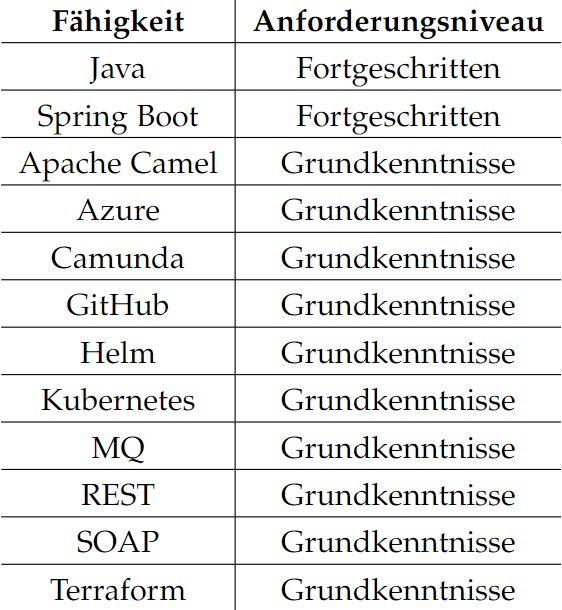
\includegraphics[width=0.5\textwidth]{gfx/projekt-1.png}\label{fig:methodik:abb2:1}}
    \subfloat[Projekt 2]{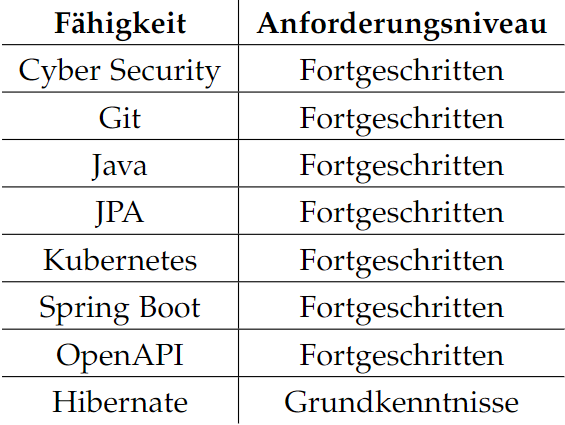
\includegraphics[width=0.5\textwidth]{gfx/projekt-2.png}\label{fig:methodik:abb2:2}}\\
    \subfloat[Projekt 3]{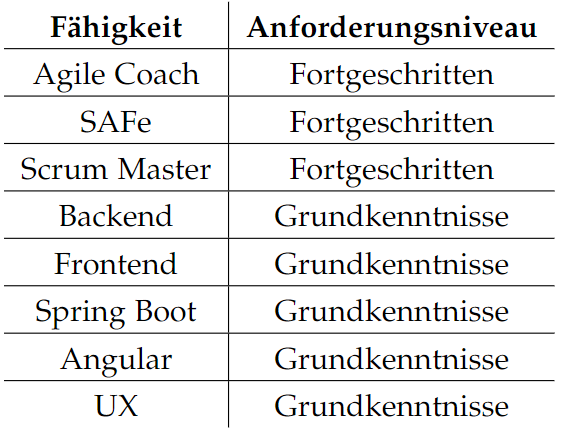
\includegraphics[width=0.5\textwidth]{gfx/projekt-3.png}\label{fig:methodik:abb2:3}}
    \subfloat[Projekt 4]{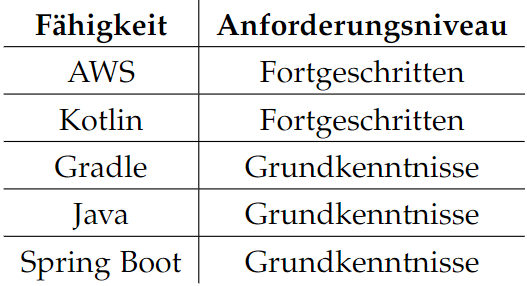
\includegraphics[width=0.5\textwidth]{gfx/projekt-4.png}\label{fig:methodik:abb2:4}}\\
    \subfloat[Projekt 5]{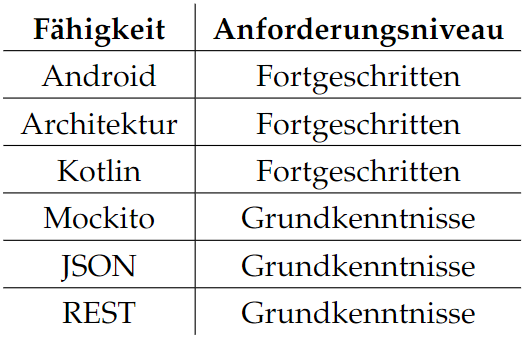
\includegraphics[width=0.5\textwidth]{gfx/projekt-5.png}\label{fig:methodik:abb2:5}}\\
\caption[Beispielprojekte des Experiments]{Beispielprojekte des Experiments}
  \label{fig:methodik:abb2}
\end{figure}

Für jede Fähigkeit eines Projekts ist ein Anforderungsniveau angegeben.
Dieses gibt an, welches Kenntnissniveau ein Mitarbeiter in der angeforderten Fähigkeit beherrschen soll.
Tabelle \ref{tab:methodik:tab1} stellt eine Beschreibung der Kenntnisse dar, die von den Fähigkeiten eines Mitarbeiters entsprechend des angeforderten Niveaus erwartet wurden.

\begin{table}[htbp]
    \begin{center}
    \begin{tabular}{p{1.5in}|p{3.25in}}
    {\textbf{Anforderungsniveau}} & {\textbf{Beschreibung}}\\
    \hline
	Grundkenntnisse & Kenntnisse entsprechen mindestens einer der Stufen "Ich habe Grundkenntnisse", "Ich habe es schon in einem Projekt eingesetzt" oder "Ich habe es in einem Projekt eingeführt" \\
    \hline
    Fortgeschritten & Kenntnisse entsprechen mindestens einer der Stufen "Ich habe Kollegen geholfen es einzusetzen", "Ich habe eine Schulung zu dem Thema gehalten" oder "Ich habe auf Konferenzen zu dem Thema Vorträge gehalten" \\
    \end{tabular}
    \end{center}
    \caption[Beschreibung des Kenntnisstands eines Mitarbeiters je Anforderungsniveau]{Beschreibung des Kenntnisstands eines Mitarbeiters je Anforderungsniveau}
	\label{tab:methodik:tab1}
\end{table}

\section{Datenerhebung}
\label{ch:methodik:datenerhebung}
In der zweiten Phase wurden die benötigten Daten erhoben.
Die Erhebung der Daten erfolgte anhand von zwei separaten Befragungen.
Die erste Befragung wurde unter den Mitarbeitern des Unternehmens durchgeführt.
Die zweite Befragung erfolgte unter den Managern des Unternehmens.
Die Befragungen wurden unabhängig von dem entwickelten Algorithmus gestaltet.
Dadurch ist eine Reproduzierbarkeit der Ergebnisse und deren Vergleichbarkeit mit Ergebnissen alternativer Algorithmen möglich.

\subsection{Befragung der Mitarbeiter}
\label{ch:methodik:datenerhebung:1}
Die Befragung unter den Mitarbeitern hatte zwei Erkenntnisse zum Ziel.
Zum einen sollte die Umfrage Auskunft über die Fähigkeiten und Präferenzen eines befragten Mitarbeiters liefern.
Zum anderen sollte über die Umfrage die Zufriedenheit eines Mitarbeiters mit den jeweiligen Beispielprojekten aus Tabelle \ref{fig:methodik:abb2} erhoben werden.

Für die Erhebung der Fähigkeiten wurden die Angestellten in der Umfrage gebeten, ihr Kenntnisniveau für jede der insgesamt 31 unterschiedlichen Fähigkeiten der Beispielprojekte anzugeben.
Zur Einordnung der Fähigkeiten wurde eine dreistufige Likert-Skala gewählt, anhand derer die Mitarbeiter ihr Kenntnisniveau angeben sollten.
Die Likert-Skala umfasste die Optionen "Keine Kenntnisse", "Grundkenntnisse" und "Fortgeschritten".
Die Optionen "Grundkenntnisse" und "Fortgeschritten" der Skala wurden entsprechend der Skala des Anforderungsniveaus der Fähigkeiten der Beispielprojekte gewählt (Vgl. Tabelle \ref{tab:methodik:tab1}).
Zusätzlich zu den Kenntnisniveaus "Grundkenntnisse" und "Fortgeschritten" konnten die Mitarbeiter darüber hinaus über die Option "Keine Kenntnisse" angeben, wenn sie eine Fähigkeit nicht beherrschten.
Abbildung \ref{fig:methodik:abb3} stellt einen Auszug aus der Umfrage zur Erhebung der Fähigkeiten eines Mitarbeiters dar.

\begin{figure}[H]
    \centering
	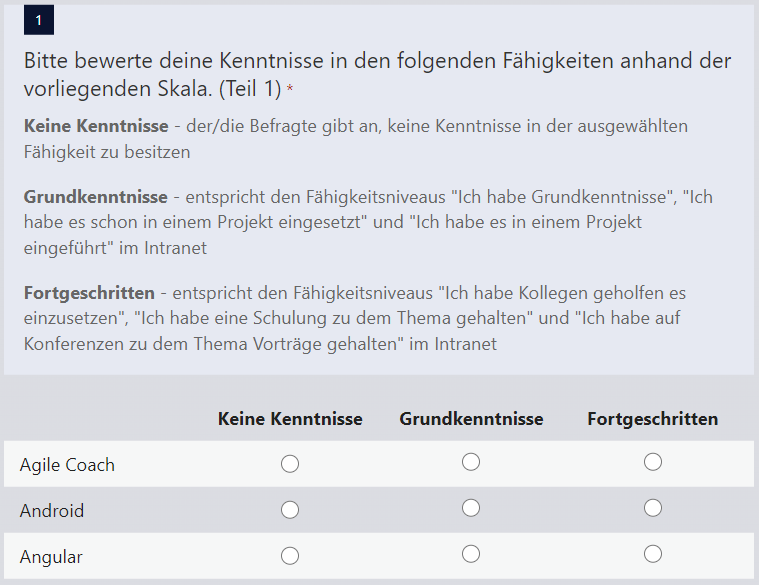
\includegraphics[width=1\textwidth]{gfx/befragung-faehigkeiten.png}
	\caption[Auszug aus der Befragung der Mitarbeiter zu ihren Fähigkeiten]{Auszug aus der Befragung der Mitarbeiter zu ihren Fähigkeiten}
	\label{fig:methodik:abb3}
\end{figure}

Für die Erhebung der Präferenzen sollten die Mitarbeiter darüber hinaus für jede der Fähigkeiten angeben, ob Interesse besteht diese in zukünftigen Projekten anzuwenden.
Hierfür wurden die Befragten aufgefordert ihr Interesse auf einer dreistufigen Likert-Skala mit den Optionen "Möchte ich anwenden", "Möchte ich nicht anwenden" und "Neutral" einzuordnen.
Eine Beschreibung der Bedeutung der Einordnung des Interesses eines Mitarbeiters für eine Fähigkeit anhand der Skala ist in Tabelle \ref{tab:methodik:tab2} dargestellt.

\begin{table}[htbp]
    \begin{center}
    \begin{tabular}{p{1.5in}|p{3.25in}}
    {\textbf{Präferenzangabe}} & {\textbf{Bedeutung}}\\
    \hline
	Möchte ich anwenden & Bei dem Mitarbeiter besteht Interesse die ausgewählte Fähigkeit in zukünftigen Projekten (weiter) anzuwenden \\
    \hline
    Möchte ich nicht anwenden & Der Mitarbeiter möchte die Fähigkeit in zukünftigen Projekten (vorerst) nicht anwenden \\
    \hline
    Neutral & Der Mitarbeiter steht der Option, die ausgewählte Fähigkeit in zukünftigen Projekten anzuwenden, neutral gegenüber \\
    \end{tabular}
    \end{center}
    \caption[Bedeutung der unterschiedlichen Ausprägungen der Likert-Skala für die Präferenzangabe]{Bedeutung der unterschiedlichen Ausprägungen der Likert-Skala für die Präferenzangabe}
	\label{tab:methodik:tab2}
\end{table}

Die Skala wurde so gewählt, dass für Mitarbeiter neben präferierten Fähigkeiten auch deren negative Präferenzen erhoben werden konnten, sowie die Fähigkeiten, denen sie indifferent gegenüberstanden.
In Abbildung \ref{fig:methodik:abb4} ist einen Auszug aus der Umfrage zur Erhebung der Präferenzen eines Mitarbeiters abgebildet.

\begin{figure}[H]
    \centering
	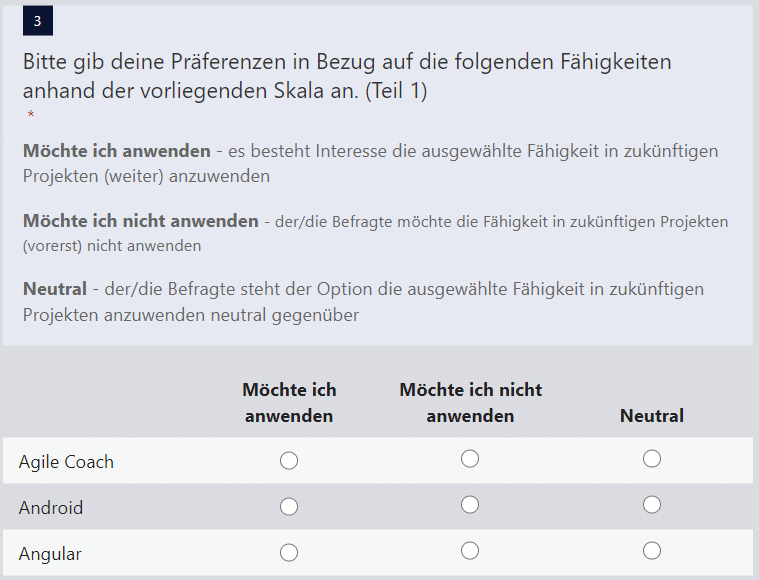
\includegraphics[width=1\textwidth]{gfx/befragung-praeferenzen.png}
	\caption[Auszug aus der Befragung der Mitarbeiter zu ihren Präferenzen]{Auszug aus der Befragung der Mitarbeiter zu ihren Präferenzen}
	\label{fig:methodik:abb4}
\end{figure}

Abschließend wurden die Mitarbeiter bezüglich ihrer Zufriedenheit mit den fünf Beispielprojekten befragt.
Hierfür wurden die Befragten aufgefordert ihre Zufriedenheit mit jeweiligen Beispielprojekt entlang einer vierstufigen ordinalen Skala anzugeben, wobei die niedrigste Angabe 1 für "Gar nicht zufrieden" und die höchste Angabe 4 für "Voll und Ganz zufrieden" stand.
Die Skala wurde bewusst so gewählt, dass Mitarbeiter keine neutrale Bewertung bezüglich ihrer Zufriedenheit abgeben konnten.
Ein Auszug der Befragung der Mitarbeiter zu ihrer Zufriedenheit ist beispielhaft für Projekt 1 in Abbildung \ref{fig:methodik:abb5} illustriert.

\begin{figure}[H]
    \centering
	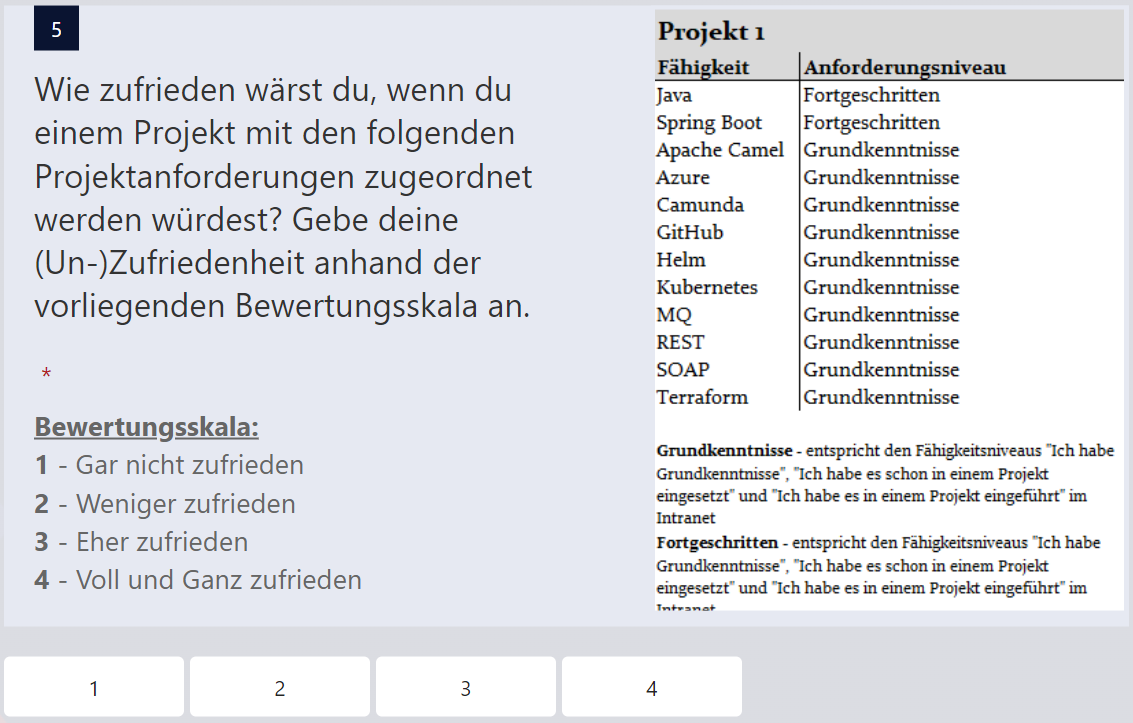
\includegraphics[width=1\textwidth]{gfx/befragung-zufriedenheit.png}
	\caption[Auszug aus der Befragung der Mitarbeiter zu ihrer Zufriedenheit mit Projekt 1]{Auszug aus der Befragung der Mitarbeiter zu ihrer Zufriedenheit mit Projekt 1}
	\label{fig:methodik:abb5}
\end{figure}

% 1. Mitarbeiter befragen nach Selbsteintschätzung der Fähigkeiten in Anlehnung an Intranet (da im Intranet nur z.T. vollständig), sowie Präferenzen (pos. und neg.)

\subsection{Befragung der Manager}
\label{ch:methodik:datenerhebung:2}
Die zweite Umfrage erfolgte unter Managern des Unternehmens und galt der Ermittlung der zu erwarteten Arbeitsleistung der Mitarbeiter in den jeweiligen Beispielprojekten.

Für die Erhebung wurden die Befragten aufgefordert für jedes der Beispielprojekte die Mitarbeiter auszuwählen, von denen sie eine hohe Arbeitsleistung erwarten würden.
Auswählen konnten die Manager aus einer Liste an Angestellten, die zuvor an der Befragung der Mitarbeiter teilgenommen hatten.
Zu jedem Angestellten wurde den Managern als Information deren Namen, Fähigkeitsbewertung und Präferenzen zur Verfügung gestellt.
Da die erhobenen Daten der Mitarbeiterbefragung zu Fähigkeiten und Präferenzen folglich als Input für die Befragung der Manager verwendet wurden, fanden die Befragungen zeitlich versetzt voneinander statt.

Für die Auswahl der Mitarbeiter mit zu erwartend hoher Arbeitsleistung wurde eine Mehrfachauswahl gewählt.
Dies sollte sicherstellen, dass als Ergebnis der Managerbefragung für jeden Mitarbeiter ein boolescher Wert vorlag, der eindeutig bestimmt, ob eine hohe Arbeitsleistung von dem jeweiligen Mitarbeiter erwartet wird oder nicht.
Abbildung \ref{fig:methodik:abb6} zeigt einen Auszug aus der Managerbefragung zu der erwarteten Arbeitsleistung der Angestellten seitens der Manager am Beispiel von Projekt 4.
Aus Datenschutzgründen wurden die Mitarbeiter in der Abbildung pseudonymisiert.

\begin{figure}[H]
    \centering
	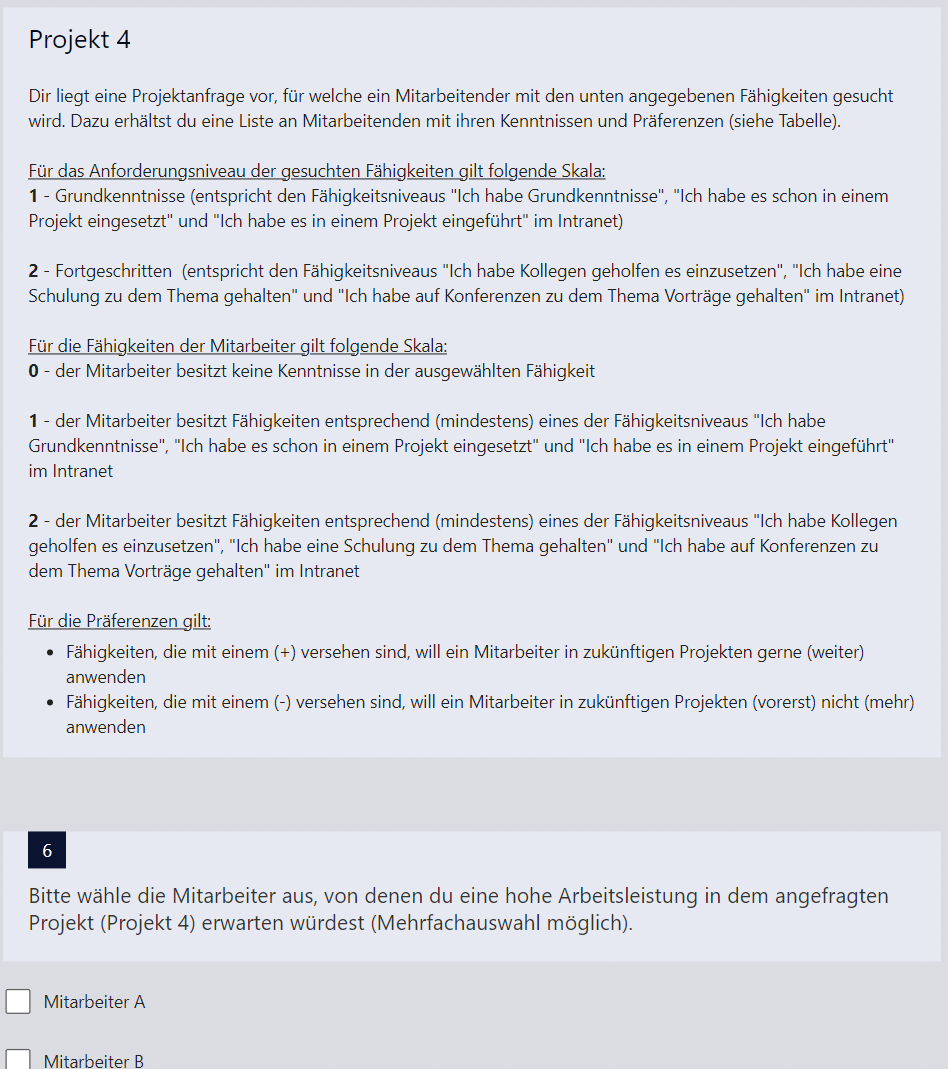
\includegraphics[width=1\textwidth]{gfx/befragung-arbeitsleistung.png}
	\caption[Auszug aus der Befragung der Manager zu der erwarteten Arbeitsleistung der Mitarbeiter in Projekt 4]{Auszug aus der Befragung der Manager zu der erwarteten Arbeitsleistung der Mitarbeiter in Projekt 4}
	\label{fig:methodik:abb6}
\end{figure}

In Abbildung \ref{fig:methodik:abb7} ist beispielhaft ein Auszug der zugehörigen Auswahlliste an Mitarbeitern dargestellt, die einem Manager in Abhängigkeit der angeforderten Fähigkeiten je Projekt zur Verfügung gestellt wurden.

\begin{figure}[H]
    \centering
	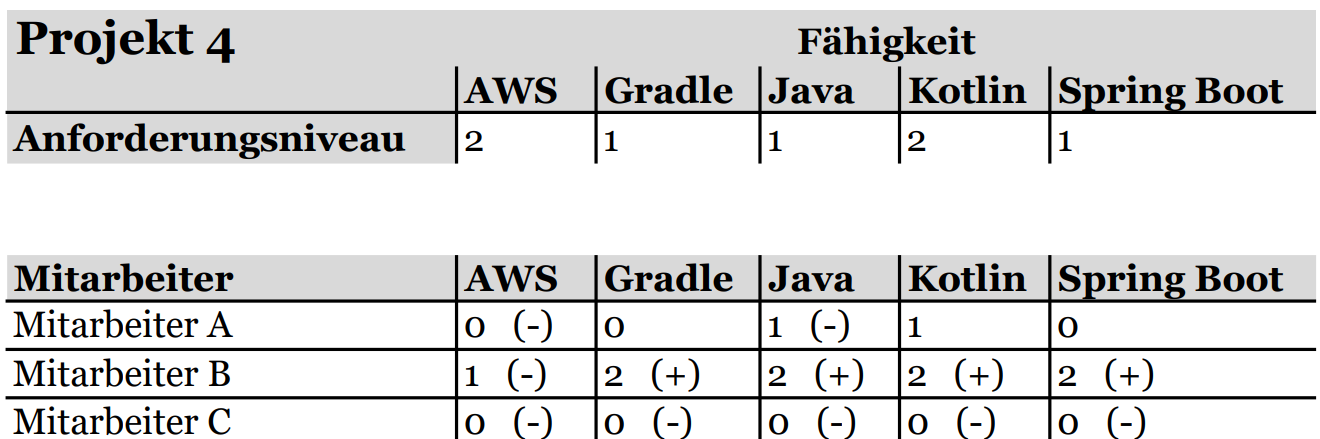
\includegraphics[width=0.95\textwidth]{gfx/befragung-arbeitsleistung-liste-ma.png}
	\caption[Auszug aus der Auswahlliste an Mitarbeitern für die Manager am Beispiel von Projekt 4]{Auszug aus der Auswahlliste an Mitarbeitern für die Manager am Beispiel von Projekt 4}
	\label{fig:methodik:abb7}
\end{figure}

\section{Auswertung des Experiments}
In der dritten Phase erfolgte die Auswertung des Feldexperiments.
In dem Kontext wurde ein multi-kriterielles Empfehlungssystem für die Empfehlung von passenden Mitarbeitern für offene Projektpositionen anhand von Fähigkeiten und Präferenzen entwickelt.

\subsection{Aufbau des Empfehlungssystems}
Für die Gestaltung des Empfehlungssystems wurde nach dem Aggregation Function Ansatz vorgegangen, welcher in Kapitel \ref{ch:erweiterungen:loesungen:modellbasiert} vorgestellt wurde.
Dieser ist unabhängig von der jeweiligen Vorhersage-Technik eines Empfehlungssystems.
Da die Bewertungen der Mitarbeiter zu ihren Fähigkeiten und Präferenzen als gegeben angenommen wurden, wurde auf eine separate Vorhersage von Fähigkeits- und Präferenzbewertungen in dieser Arbeit verzichtet.
Der Aggregation Function Ansatz eignet sich daher besonders, da das nachfolgend vorgestellte Verfahren in Verbindung mit jeder beliebigen Vorhersage-Technik angewandt werden kann.

Das Empfehlungssystem wurde so konzipiert, dass Entscheidungsträger (Manager) die Nutzer des Systems darstellen.
Elemente des Empfehlungssystems sind die Mitarbeiter, die den Entscheidungsträgern für Projektpositionen vorgeschlagen werden können.
Die Nutzer des Systems werden in Form einer offenen Projektposition repräsentiert, welche als Sammlung der angeforderten Fähigkeiten der Projektposition abgebildet werden können.
Jedes Element des Systems wird durch seine Fähigkeiten und Präferenzen dargestellt.
Unter der Bedürfniserfüllung eines Nutzers (Entscheidungsträgers) durch ein Element (Mitarbeiter) wird in dem System die Erfüllung der angeforderten Fähigkeiten der Projektposition eines Nutzers durch die Fähigkeiten eines Elements verstanden.
In Anlehnung an \textcite[S. 207ff.]{pizzato:2010} wird dieser Präferenzwert als Fähigkeits-Kompatibilität bezeichnet.
Unter der Bedürfniserfüllung eines Elements durch einen Nutzer wird die Erfüllung der präferierten Fähigkeiten eines Elements durch die angeforderten Fähigkeiten der Projektposition eines Nutzers verstanden.
Analog wird der Präferenzwert eines Mitarbeiters für einen Entscheidungsträger als Präferenz-Kompatibilität bezeichnet.

In dem Empfehlungssystem wurde ein biltareraler Algorithmus für die Zuordnung von Mitarbeitern zu Projektpositionen implementiert.
Als Benchmark wurde anhand derselben Vorgehensweise ein unilateraler Algorithmus für die Zuordnung von passenden Mitarbeitern zu Projektpositionen aufgesetzt.
Die beiden Algorithmen unterscheiden sich lediglich in den Kriterien, die für die Zuordnung herangezogen werden.
So erfolgt die Zuordnung über den unilateralen Algorithmus anhand der Fähigkeits-Kompatibilität, während die bilaterale Zuordnung neben der Fähigkeits-Kompatibilität auch die Präferenz-Kompatibilität miteinbezieht.
In Anlehnung an die Darstellung des Konzepts wechselseitiger Empfehlungen in Abbildung \ref{fig:empfehlungssysteme:rrs:abb2} ist in Abbildung \ref{fig:methodik:abb9} das Konzept der uni- und bilateralen Empfehlung in dem entwickelten System dargestellt.

\begin{figure}[H]
    \centering
	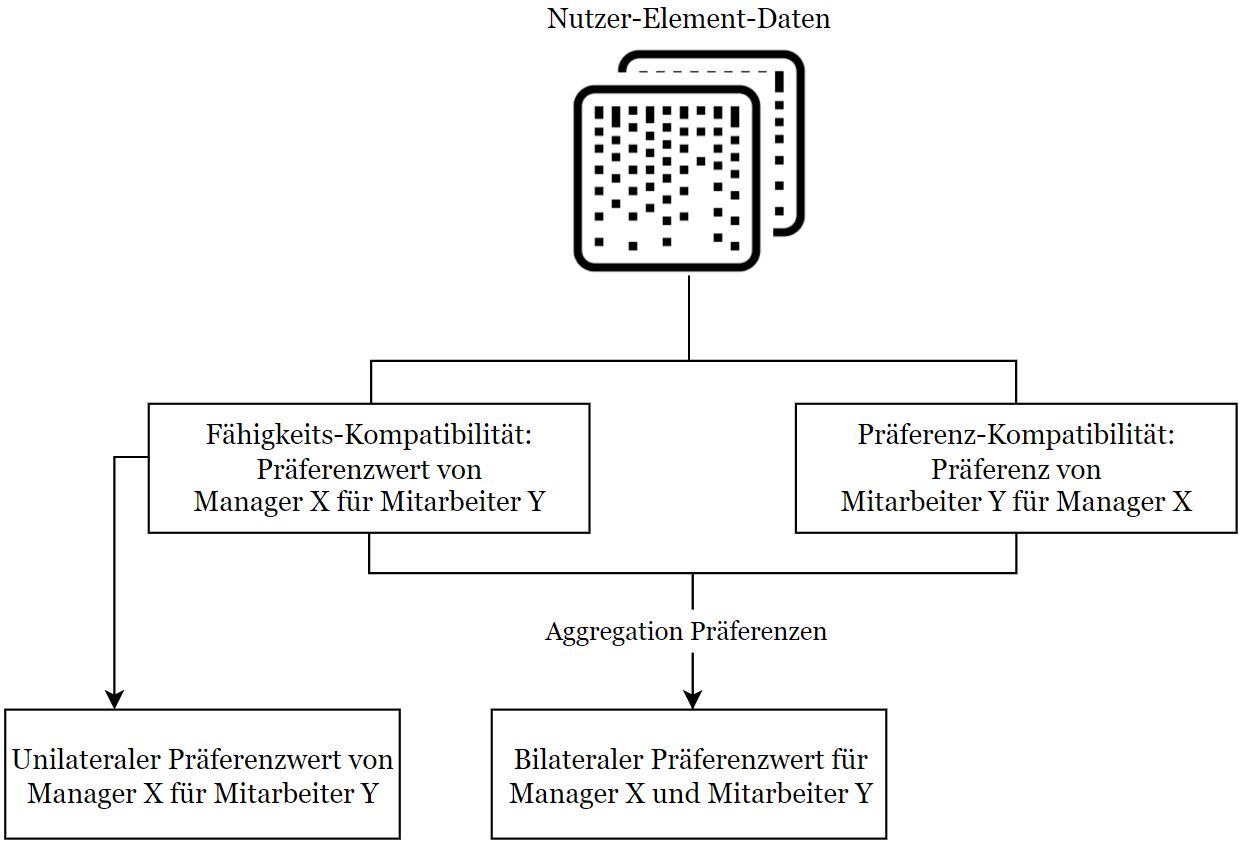
\includegraphics[width=1.0\textwidth]{gfx/concept-rrs-in-praxis.png}
	\caption[Konzept der der uni- und bilateralen Empfehlung]{Konzept der uni- und bilateralen Empfehlung}
	\label{fig:methodik:abb9}
\end{figure}

Die beiden Algorithmen wurden in einen Microservice eingebettet, welcher nachfolgend als Empfehlungsservice bezeichnet wird.
Der Empfehlungsservice stellt eine POST-Schnittstelle zur Verfügung, über die Manager für offene Projektpositionen passende Mitarbeiter vorgeschlagen bekommen können.
Der Dienst wurde in der Programmiersprache Python implementiert, wobei für das Erstellen der Webanwendung das Framework Flask verwendet wurde.
% Die Berechnungen wurden unter Anwendung der Bibliothek Numpy entwickelt.
Der Service wird als Docker-Container bereitgestellt.
Abbildung \ref{fig:methodik:abb8} zeigt eine vereinfachte Darstellung des Dienstes.

\begin{figure}[H]
    \centering
	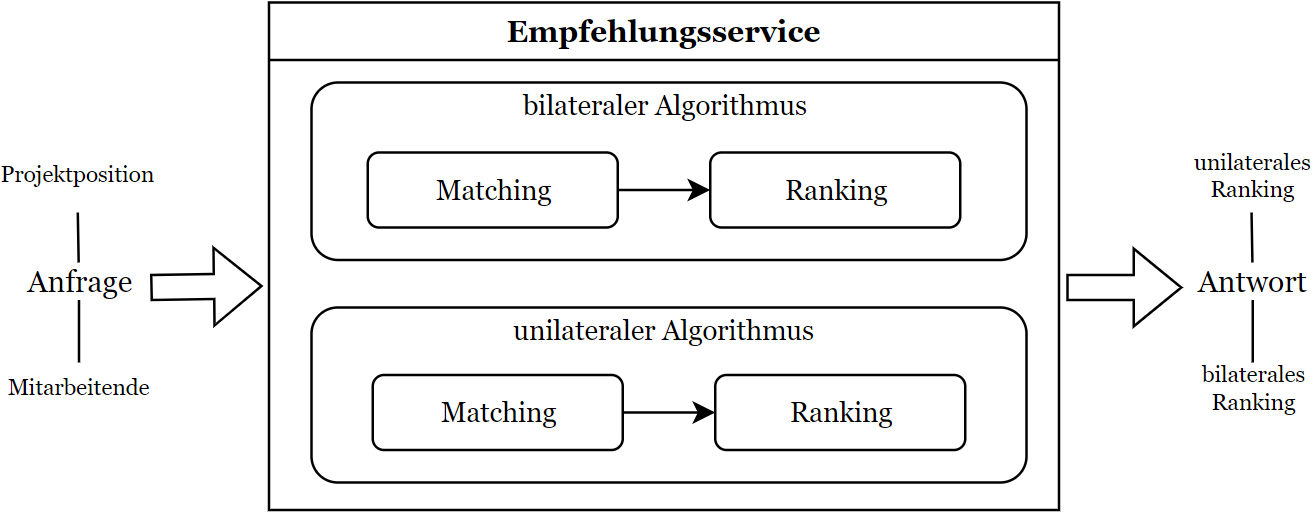
\includegraphics[width=1.0\textwidth]{gfx/empfehlungsservice.png}
	\caption[Aufbau des Empfehlungsservice]{Aufbau des Empfehlungsservice}
	\label{fig:methodik:abb8}
\end{figure}

Wie der Abbildung entnommen werden kann, akzeptiert der Dienst Anfragen, die im Body die angefragte Projektposition sowie die zur Verfügung stehenden Mitarbeiter enthalten.
Diese Daten werden in Form eines JSON-Arrays an den Service übermittelt.
In Listing \ref{lst:methodik:lst1} ist eine solche Anfrage beispielhaft abgebildet.

\lstinputlisting[
    language=json,
    caption=Beispiel einer Anfrage an den Empfehlungsservice,
    captionpos=b,
    label=lst:methodik:lst1
    ]{gfx/request-body.json}

Eine Projektposition wird in Form einer Liste an angeforderten Fähigkeiten (\textit{skills}) dargestellt.
Jede angeforderte Fähigkeit kann über einen Namen und ein zugehöriges Anforderungsniveau (\textit{level}) beschrieben werden.
Das Anforderungsniveau ist als Integer codiert, wobei eine 1 dem Anforderungsniveau "Grundkenntnisse" und eine 2 dem Anforderungsniveau "Fortgeschritten" entspricht.
Die zur Verfügung stehenden Mitarbeiter werden als Liste dargestellt.
Ein Mitarbeiter wird eindeutig über seine Mailadresse identifiziert und verfügt über eine Liste an Fähigkeiten (\textit{skills}) mit zugehörigem Kenntnisniveau (\textit{level}) sowie einer Liste an Präferenzen (\textit{preferences}) mit zugehörigem Präferenzniveau (\textit{level}).
Die Ausprägungen "Grundkenntnisse" und "Fortgeschritten" des Kenntnisniveaus sind analog zum Anforderungsniveau kodiert.
Zusätzlich ist das Kenntnisniveau "Keine Kenntnisse" als Zahl 0 kodiert.
Die Präferenzangabe ist ebenfalls als Integer kodiert, wobei "Möchte ich anwenden" einer 1, "Möchte ich nicht anwenden" einer -1 und "Neutral" einer 0 entspricht.

Als Ergebnis produziert der Service zwei Listen: eine Liste mit empfohlenen Mitarbeitern basierend auf dem bilateralen Algorithmus und eine Liste mit empfohlenen Mitarbeitern durch den unilateralen Algorithmus.
Beide Listen sind absteigend sortiert und stellen ein Ranking der Mitarbeiter dar.
Die Liste des bilateralen Algorithmus sortiert die Angestellten anhand ihres bilateralen Präferenzwertes, während der unilaterale Algorithmus die Mitarbeiter anhand ihres unilateralen Präferenzwertes sortiert.
Beide Listen schickt der Service in einer Antwort an den Client zurück.
Hierbei wird jeder Mitarbeiter durch seine Mailadresse und seinen Präferenzwert (\textit{matchValue}) abgebildet.
In Listing \ref{lst:methodik:lst2} ist beispielhaft die Rückgabe des Empfehlungsservice für die Anfrage aus Listing \ref{lst:methodik:lst1} dargestellt.

\lstinputlisting[
    language=json,
    caption=Beispiel einer Antwort des Empfehlungsservice,
    captionpos=b,
    label=lst:methodik:lst2
    ]{gfx/response-body.json}

Für die Ermittlung der uni- und bilateralen Kompatibilitätswerte wurden zwei Algorithmen implementiert.
% Die erste Liste stellt eine sortierte Liste der Mitarbeitenden dar, die anhand des bilateralen Algorithmus ermittelt wurden.
% Dieses sollte in der Lage sein, aus einer Menge an zu Verfügung stehenden Mitarbeitenden die fünf passensten Mitarbeitenden anhand eines unilateralen und anhand eines bilateralen Algorithmus zu empfehlen.

% Aufteilen der Daten in Trainings- und Testdaten
% Nutzen der Trainingsdaten, um Gewichte des bilateralen Algorithmus zu lernen
% Vergleich des entwickelten bilateralen Algorithmus mit einer unilateralen Variante anhand der Testdaten

\subsection{Gestaltung des bilateralen Algorithmus}
Wie Abbildung \ref{fig:methodik:abb8} zeigt, kann die Logik des bilateralen Algorithmus in zwei Kernfunktionalitäten aufgeteilt werden: Matching und Ranking.
Das Matching umfasst die Kalkulation der Präferenzwerte der Mitarbeiter mit der angeforderten Projektposition.
Das Ranking beinhaltet das Sortieren der Mitarbeiter anhand ihres Präferenzwertes (siehe Abbildung \ref{fig:methodik:abb8}).
Nachfolgend wird erläutert, wie die Funktionalitäten umgesetzt wurden.

\subsubsection{Konzeption von Fähigkeiten und Präferenzen}
Im Matching-Teil des Algorithmus wird für jeden Mitarbeiter ermittelt, wie sehr dessen Fähigkeiten und dessen Präferenzen mit den angeforderten Fähigkeiten im Projekt übereinstimmen.
Hierfür ermittelt der Algorithmus in Anlehnung an \textcite[S. 207ff.]{pizzato:2010} zwei separate Kompatibilitätswerte.
Für die Berechnung der Präferenz-Kompatibilität wurde nach dem Verfahren von \textcite[S. 269ff.]{pizzato:2:inproceedings} für die Kombination positiver und negativer Präferenzen vorgegangen, welches in Kapitel \ref{ch:verwandte_arbeiten:1} vorgestellt wurde.
Demnach kann die Präferenz-Kompatibilität $C_{Pref}^{\pm}(c,s)$ eines Mitarbeiters $s$ mit einer angeforderten Projektposition $c$ wie folgt ermittelt werden:
\begin{equation}\label{methodik:eq:1}
    C_{Pref}^{\pm}(c,s)=\frac{1+C_{Pref}^{+}(c,s)-C_{Pref}^{-}(c,s)}{2}
\end{equation}
Die positive Präferenz-Kompatibilität $C_{Pref}^{+}(c,s)$ eines Mitarbeiters mit einem Projekt ermittelt der Algorithmus, indem die Anzahl der angeforderten Fähigkeiten, die ein Mitarbeiter präferiert durch die Gesamtzahl an angefragten Fähigkeiten geteilt wird:
\begin{equation}\label{methodik:eq:2}
    C_{Pref}^{+}(c,s)=\frac{\sum\limits_{i \in F_{c}} \mathbb{1}_{i \in P_{s}}}{|F_{c}|}
\end{equation}
In Gleichung \ref{methodik:eq:2} stellt $F_{c}$ die Menge an angeforderten Fähigkeiten einer Projektposition dar, während $P_{s}$ die Menge an Fähigkeiten repräsentiert, die ein Mitarbeiter präferiert.

Die Kalkulation der negativen Präferenz-Kompatibilität $C_{Pref}^{-}(c,s)$ erfolgt analog zu Gleichung \ref{methodik:eq:2}, indem die Anzahl an Fähigkeiten, die ein Mitarbeiter nicht anwenden möchte durch die Gesamtzahl an angefragten Fähigkeiten geteilt wird.
Da Fähigkeiten, denen ein Angestellter neutral gegenübersteht, weder zu einem höheren noch zu einem niedrigeren Rang eines Mitarbeiters im Ranking führen sollen, werden diese bei der Kalkulation der Präferenz-Kompatibilität nicht berücksichtigt.

Für die Mitarbeiterin Jane D. der Anfrage in Listing \ref{lst:methodik:lst1} ergibt sich die Präferenz-Kompatibilität für die angeforderte Projektposition demnach wie folgt:
\begin{equation}\label{methodik:eq:4}
    C_{Pref}^{\pm}(c,Jane \textnormal{ }D.) = \frac{1+\frac{1}{1}-\frac{0}{1}}{2} = 1
\end{equation}

Für die Berechnung der Fähigkeits-Kompatibilität wurde eine abgewandelte Version des Verfahrens von \textcite[S. 269ff.]{pizzato:2:inproceedings} entwickelt.
Diese ermöglicht die Berücksichtigung einer teilweisen Erfüllung von Fähigkeiten durch einen Mitarbeiter.
Das bedeutet, der Algorithmus ist so gestaltet, dass ein Mitarbeiter, der beispielsweise eine angeforderte Fähigkeit mit Anforderungsniveau "Fortgeschritten" auf dem Niveau "Grundkenntnisse" beherrscht, eine höhere Kompatibilität aufweist als ein Mitarbeiter, der diese Fähigkeit nicht beherrscht.
Hierfür ermittelt der Algorithmus für jede angeforderte Fähigkeit deren anteilige Erfüllung durch die Kenntnisse eines Mitarbeiters.
Diese wird berechnet, indem je Fähigkeit das Kenntnisniveau eines Mitarbeiters durch das Anforderungsniveau einer angeforderten Fähigkeit dividiert wird.
Die Summe der anteiligen Fähigkeiten wird anschließend durch die Anzahl an angeforderten Fähigkeiten geteilt.
Dadurch ergibt sich für die Kalkulation der Fähigkeits-Kompatibilität des Algorithmus folgende Formel:
\begin{equation}\label{methodik:eq:3}
    C_{Skills}(c,s)=\frac{1}{|F_{c}|} \cdot \sum\limits_{i \in F_{c}} \mathbb{1}_{i \in F_{s}} \frac{level(i \in F_{s})}{level(i \in F_{c})}
\end{equation}
In Gleichung \ref{methodik:eq:3} stellt $F_{s}$ die Menge an Fähigkeiten dar, die ein Angestellter beherrscht (Kenntnisniveaus "Grundkenntnisse" und "Fortgeschritten").
Der Ausdruck $level(i \in F_{s})$ gibt den Wert des Kenntnisniveaus einer beherrschten Fähigkeit eines Mitarbeiters an.
Analog bezeichnet $level(i \in F_{c})$ den Wert des Anforderungsniveaus einer angeforderten Fähigkeit in einem Projekt.

Da ein Mitarbeiter eine angeforderte Fähigkeit auch besser beherrschen kann als gefordert ist, musste bei der Konzeption darüber hinaus berücksichtigt werden, wie mit einer Überqualifikation eines Mitarbeiters in einer Fähigkeit verfahren wird.
Der Algorithmus wurde so gestaltet, dass eine Überqualifikation eines Mitarbeiters ($level(i \in F_{s}) > level(i \in F_{c})$) gleich gehandhabt wird, wie die exakte Erfüllung einer Fähigkeit ($level(i \in F_{s}) = level(i \in F_{c})$).
Wird eine Fähigkeit beispielsweise auf dem Niveau "Grundkenntnisse" ($\widehat{=} \textnormal{ }1$) angefordert, die ein Mitarbeiter auf dem Niveau "Fortgeschritten" ($\widehat{=} \textnormal{ }2$) beherrscht, wird für die anteilige Erfüllung eine 1 ($\frac{level(i \in F_{c})}{level(i \in F_{c})}$) anstelle einer 2 ($\frac{level(i \in F_{s})}{level(i \in F_{c})}$) angenommen.
Dadurch soll verhindert werden, dass das Fehlen einer Fähigkeit durch die Überqualifikation in einer anderen Fähigkeit kompensiert wird.
% hier beispiel einfügen für skill kompatibilitätsrechnung

Für die Mitarbeiterin Jane D. der Anfrage in Listing \ref{lst:methodik:lst1} ergibt sich die Fähigkeits-Kompatibilität demnach wie folgt:
\begin{equation}\label{methodik:eq:5}
    C_{Skills}(c,Jane \textnormal{ }D.) = \frac{1}{1} \cdot (\frac{0}{1}) = 0
\end{equation}

Für die Kombination der Fähigkeits- und Präferenz-Kompatibilität im bilateralen Algorithmus wurden verschiedene Aggregationsmethoden betrachtet.

\subsubsection{Aggregation}
Nach dem Aggregation Function Ansatz existieren verschiedene Verfahren für die Aggregation der Kriterien in einem multi-kriteriellen System.
Im Kontext wechselseitiger Empfehlungssysteme wurden verschiedene statistische Verfahren für die Aggregation der Präferenzen zweier Parteien identifiziert.
Deren Einsatz wurde in Kapitel \ref{ch:verwandte_arbeiten} diskutiert.
% Beispielrechnung in Anhang?
% Im Rahmen der verwandten Arbeiten wurden verschiedene statistische Methoden für die Aggregation beider Kriterien vorgestellt.
Bei der Entscheidung für eine Aggregationsmethode des bilateralen Algorithmus wurden lediglich Verfahren mit individueller Gewichtung der Kriterien betrachtet.
Dem lag die Annahme zugrunde, dass die Fähigkeits-Kompatibilität im Vergleich von höherer Bedeutung bei der Zuordnung von Mitarbeitern für Projekte ist als die Präferenz-Kompatibilität, da Manager die finale Entscheidung bei der Zuordnung treffen.

Obwohl das harmonische Mittel in dem Experiment von \textcite[S. 1ff.]{kumari:2:inproceedings} die besten Ergebnisse erzielen konnte, wurde sich im bilateralen Algorithmus gegen diese Methode entschieden.
Zum einen wurde in Kapitel \ref{ch:verwandte_arbeiten:1} erläutert, dass das harmonische Mittel für eine Fähigkeits- bzw. Präferenz-Kompatibilität von 0 nicht definiert ist.
FÜr den vorliegenden Anwendungsfall wurde jedoch davon ausgegangen, dass in der Praxis durchaus Mitarbeiter existieren, die keine der angeforderten Fähigkeiten einer Projektposition besitzen (Fähigkeits-Kompatibilität $= 0$) bzw. präferieren (Präferenz-Kompatibilität $= 0$).
Auch wenn eine individuelle Gewichtung der Kriterien durch das gewichtete harmonische Mittel möglich gewesen wäre, wurde sich daher gegen die Methode entschieden.
Darüber hinaus zeigten Experimente von \textcite[S. 131ff.]{kleinerman:2:inproceedings}, dass eine gewichtete Summe im Vergleich zum harmonischen Mittel zu besseren Ergebnissen führen kann.
In Anlehnung an \textcite[S. 131ff.]{kleinerman:2:inproceedings} wurde daher die gewichtete Summe als Aggregationsmethode in dem bilateralen Algorithmus umgesetzt.
Die Kombination von Fähigkeits- und Präferenz-Kompatibilität ermittelt der Algorithmus demnach wie folgt:
\begin{equation}\label{methodik:eq:6}
    PW_{c,s}^{bil}(\alpha) = \alpha \cdot C_{Skills}(c,s) + (1-\alpha) \cdot C_{Pref}^{\pm}(c,s)
\end{equation}
Das Ergebnis $PW_{c,s}^{bil}$ der Aggregation stellt den bilateralen Präferenzwert dar.

\subsubsection{Gewichtung}
\label{ch:methodik:auswertung:gewichtung}
Da die genaue Bedeutung der einzelnen Kriterien in der Zuordnung von Mitarbeitern zu Projekten nicht bekannt ist, wurde ein separates Skript zur Bestimmung eines optimalen Werts für $\alpha$ entwickelt.
Das Skript wurde in der Programmiersprache Python programmiert.
Hierfür wurden die erhobenen Daten der Mitarbeiter- und Managerbefragung herangezogen (Vgl. Kapitel \ref{ch:methodik:datenerhebung:1} und \ref{ch:methodik:datenerhebung:2}).

In Anlehnung an das in Kapitel \ref{ch:verwandte_arbeiten:1} vorgestellte Verfahren von \textcite[S. 131ff.]{kleinerman:2:inproceedings} wurde das Optimierungsproblem zur Bestimmung von $\alpha$ wie folgt definiert:
\begin{equation}\label{methodik:eq:7}
    \begin{aligned}
        \min_{\alpha} \sum_{c \in C} \sum_{s \in S} \mathbb{1}_{s \in SuccMatch_{c}} Rank_{s} (PW_{c,*}(\alpha))\\
        \textnormal{u.d.B. } 0 \leq \alpha \leq 1\\
    \end{aligned}
\end{equation}
Vereinfach gesagt wird durch die Lösung des Optimierungsproblems das Gewicht $\alpha$ so gewählt, dass für eine Menge an Mitarbeiter $S$ und eine Menge an Projekten $C$ die Summe der Ränge der Mitarbeiter, die in Projekten erfolgreich waren (d.h. $s \in SuccMatch_{c}$), möglichst minimal wird.
Das Verfahren optimiert $\alpha$ folglich dahingehend, dass Mitarbeiter, die in Projekten als erfolgreich eingestuft wurden, in der Liste an empfohlenen Angestellten an einen Manager möglichst weit oben platziert werden.
Als erfolgreich wurden Mitarbeiter eingestuft, die sowohl angaben mit einem Projekt zufrieden gewesen zu sein ("Eher zufrieden" oder "Voll und Ganz zufrieden"), als auch von mindestens einem Manager als Mitarbeiter mit hoher Arbeitsleistung eingeschätzt wurden.

Der Brent-Algorithmus zur Lösung des Optimierungsproblems aus Gleichung \ref{methodik:eq:7} wurde über die Funktion \textit{minimize\textunderscore scalar} der Bibliothek \textit{scipy.opti\-mize} in das Programm integriert.
Für $\alpha$ wurde ein Intervall von 0 bis 1 gewählt.
Anhand der erhobenen Daten der Mitarbeiter- und Managerbefragung ermittelte der Algorithmus in dem Intervall von 0 bis 1 das optimale Gewicht bei $\alpha = 0.6342$.

Für die Mitarbeiterin Jane D. der Anfrage in Listing \ref{lst:methodik:lst1} ergibt sich der bilaterale Präferenzwert demnach wie folgt:
\begin{equation}\label{methodik:eq:9}
    PW_{c,Jane \textnormal{ }D.}^{bil}(0.6342) = 0.6342 \cdot 0 + (1-0.6342) \cdot 1 = 0.3658
\end{equation}

Im Unterschied zum bilateralen Algorithmus wird für die Zuordnung von Mitarbeitern zu Projekten im unilateralen Algorithmus als einziges Kriterium die Fähigkeits-Kompatibilität herangezogen.
Im unilateralen Algorithmus wird der Präferenzwert demnach wie folgt ermittelt:
\begin{equation}\label{methodik:eq:8}
    PW_{c,s}^{unil} = C_{Skills}(c,s)
\end{equation}
Die Schritte Aggregation und Gewichtung waren folglich für die Implementierung des unilateralen Algorithmus nicht von Belangen.
Der unilaterale Präferenzwert für die Mitarbeiterin Jane D. der Anfrage in Listing \ref{lst:methodik:lst1} ergibt sich demnach wie folgt:
\begin{equation}\label{methodik:eq:10}
    PW_{c,Jane \textnormal{ }D.}^{unil} = 0
\end{equation}

% Ermitteln der Gewichte: alpha so wählen, dass Endergebnis möglichst optimal -> bedeutet für uns: zufriedene und leistungsfähige Mitarbeiter werden empfohlen -> erscheinen oben im Ranking
% Ziel: Gegeben einer Funktion f, welches von ein oder mehreren Input-Variablen abhängt, finden der Ausprägungen der Input-Variablen, für die f minimal wird. Obacht: f umfasst hier mehr als nur rws, da auch das ranking danach miteinbezogen wird -> zu minimieren ist die Summe der Ränge der zufriedenen und Leistungsfähigen MA über alle Projekte hinweg
% Hier: mithilfe des Brent Algorithmus in anlehnung an die verwandte Arbeit von \textcite[S. 131ff.]{kleinerman:2:inproceedings}
% Nach https://e-maxx.ru/bookz/files/numerical_recipes.pdf S. 489 gibt es keinen perfekten Optimierungs-Algorithmus -> daher ist es grundsätzlih ratsam, verschiedene Techniken auszuprobieren und zu vergleichen.
% Was macht der Brent Algorithmus?: % https://users.wpi.edu/~walker/MA3257/HANDOUTS/brents_algm.pdf

% \begin{itemize}
% 	\item In Essenz einfach eine Strategie für das Finden von lokalen Minima ohne Ableitung, indem sich von einem Intervall iterativ an ein Minima angenähert wird, entweder über GSS oder über SPI % file://wsl%24/Ubuntu/home/masc6/Projects/masterarbeit/literatur/Minimization%20or%20Maximization%20of%20Functions.pdf
% 	\item Unterscheiden zw. Brent Methode für root search und Brent-Methode für Minimasuche ohne Derivate (Ableitung)
% 	\item Kombination von successive parabolic interpolation (schnell) und golden-section search (garantiertes finden von Minimum) % für Erklärung siehe video hier: https://www.youtube.com/watch?v=BQm7uTYC0sg
% \end{itemize}

% Lösung über Python Skript unter Einsatz der scipy-Bibliothek (siehe Anhang).
% minimize_scalar function für das Finden von Minima einer skalaren Funktion (output eines einzelnen Wertes) mit einer Variablen (in unserem Fall alpha), deren default Methode brent ist
% Angeben eines Intervalls (hier: zwischen 0 und 1)
% Beschreibung des Algorithmus in anlehung an file://wsl%24/Ubuntu/home/masc6/Projects/masterarbeit/literatur/Minimization%20or%20Maximization%20of%20Functions.pdf ggf. in den Anhang?


% im ersten Schritt identifiziert, welche Eingangsdaten der Algorithmus erhält und welche Ausgangsdaten erwartet werden.
% Wie aus Listing \ref{lst:methodik:lst1} hervorgeht, liegen die Projektpositionen in Form einer Liste an Fähigkeiten vor.

% Für die Gestaltung des Algorithmus wurden die im Rahmen der Befragungen erhobenen Daten in Trainings- und Testdaten unterteilt.

% \section{Aufbau des Empfehlungssystems}
% Microservice-Architektur -> Empfehlungs-komponente (Rankings)

\subsection{Ablauf der Evaluation}
\label{ch:methodik:auswertung:ablauf}
Für die Auswertung des Experiments sollte für die fünf Beispielprojekte verglichen werden, wie sich der Einsatz der jeweiligen Algorithmen auf die Zufriedenheit und die Arbeitsleistung der empfohlenen Mitarbeiter auswirkt.
Da erhobene Daten für die Ermittlung des Gewichts $\alpha$ im bilateralen Algorithmus benötigt wurden, wurde sich für die Auswertung des Experiments für eine Aufteilung der Daten in Trainings- und Testdaten entschieden.
Dadurch sollte verhindert werden, dass dieselben Daten, für die der bilaterale Algorithmus optimiert wurde, zugleich für die Evaluation desselbigen verwendet werden.

Für die Aufteilung wurde jeder Datensatz mit einer eindeutigen Identifikationsnummer versehen.
Anhand der Identifikationsnummer wurden zufällig 75 Prozent der Datensätze ausgewählt und für das Training verwendet.
Die übrigen 25 Prozent der Datensätze wurden als Testdaten herangezogen.

Um eventuell auftretenden Bias bei der zufälligen Aufteilung der Datensätze in Trainings- und Testdaten zu vermeiden, wurde das zufällige Aufteilen insgesamt fünf mal wiederholt.
Dadurch entstanden fünf Trainings- und fünf zugehörige Test-Samples.
Der entwickelte bilaterale Algorithmus wurde für jede der 5 Sample-Datensätze evaluiert.

Nach dem vorgestellten Verfahren in Abschnitt \ref{ch:methodik:auswertung:gewichtung} wurde für jedes Sample basierend auf den Trainingsdaten das optimale Gewicht $\alpha$ näherungsweise bestimmt.
Dieses Gewicht wurde im Anschluss an den bilateralen Algorithmus übergeben.
Anhand der Mitarbeiter des Testdatensatzes eines jeden Samples wurde daraufhin für jedes Projekt einmal anhand des uni- und einmal anhand des bilateralen Algorithmus ein Ranking der fünf passensten Mitarbeiter ermittelt.

Um die Auswirkungen des bilateralen Algorithmus auf die Zufriedenheit der Angestellten zu ermitteln, wurde die Genauigkeit der Empfehlungen unter Anwendung des jeweiligen Algorithmus bestimmt.
Für die Bestimmung der Genauigkeit des jeweiligen Algorithmus wurde in jedem Projekt innerhalb eines Samples die Mitarbeiter des unilateralen sowie des bilateralen Rankings ermittelt, die angaben mit dem jeweiligen Projekt zufrieden zu sein ("Eher zufrieden" und "Voll und ganz zufrieden").
Daraufhin wurde der Anteil an zufriedenen Mitarbeitern unter den fünf empfohlenen Angestellten je Ranking ermittelt und miteinander verglichen.
Die Veränderung des Anteils des bilateralen Rankings im Vergleich zum unilateralen Ranking diente als Indikator dafür, ob die Zufriedenheit stieg, sank oder gleich blieb.

Für die Ermittlung der Auswirkung des bilateralen Algorithmus auf die Arbeitsleistung der Mitarbeiter wurde analog zu der Zufriedenheit vorgegangen.
Hierbei wurden die Anteile jedoch anhand der Mitarbeiter des unilateralen bzw. des bilateralen Rankings ermittelt, deren Arbeitsleistung von mindestens einem Manager in dem jeweiligen Projekt als hoch eingestuft wurde.


% durfte nicht dasselbe Gewicht genommen werden, wohin das system auch optimiert wurde, daher samples mit jeweils separater ermittlung der gewichte und dann anwenden auf testdaten

\shorthandon{"}